% Tikz File 'fig_03_wikibaseGraph.tex'
\documentclass{standalone}
\usepackage{tikz}
\usepackage{../mystyle}
\newcommand{\myfont}[1]{\ensuremath{\mathcal{#1}}}

\newcommand{\triple}[3]{\ensuremath{\langle #1,#2,#3 \rangle}}
\newcommand{\quadruple}[4]{\ensuremath{\langle #1,#2,#3,#4\rangle}}

\newcommand{\ItemSet}{\myfont{Q}}
\newcommand{\PropSet}{\myfont{P}}
\newcommand{\EntitySet}{\myfont{E}}
\newcommand{\ValueSet}{\myfont{V}}
\newcommand{\DataValueSet}{\myfont{D}}
\newcommand{\StmtSet}{\rho}
\newcommand{\FinSet}[1]{\ensuremath{FinSet(#1)}}

\newcommand{\hrefc}[3][blue]{\href{#2}{\color{#1}{#3}}}%

\newcommand{\elemento}[2]{\ensuremath{\hrefc[violet]{http://www.wikidata.org/entity/#2}{#1}}}
\newcommand{\propiedad}[2]{\ensuremath{\hrefc[blue]{http://www.wikidata.org/entity/#2}{#1}}}
\newcommand{\alanTuring}{\elemento{alanTuring}{Q7251}}
\newcommand{\wilmslow}{\elemento{wilmslow}{Q2011497}}
\newcommand{\town}{\elemento{town}{Q3957}}
\newcommand{\government}{\elemento{government}{Q220798}}
\newcommand{\warringtonLodge}{\elemento{warringtonLodge}{Q20895942}}
\newcommand{\bombe}{\elemento{bombe}{Q480476}}
\newcommand{\unitedKingdom}{\elemento{unitedKingdom}{Q145}}
\newcommand{\computer}{\elemento{computer}{Q11742076}}
\newcommand{\dateOfBirth}{\propiedad{dateOfBirth}{P569}}
\newcommand{\placeOfBirth}{\propiedad{placeOfBirth}{P19}}
\newcommand{\country}{\propiedad{country}{P27}}
\newcommand{\employer}{\propiedad{employer}{P108}}
\newcommand{\discoverer}{\propiedad{discoverer}{P61}}
\newcommand{\dateOfDeath}{\propiedad{dateOfDeath}{P570}}
\newcommand{\placeOfDeath}{\propiedad{placeOfDeath}{P20}}
\newcommand{\timeStart}{\propiedad{timeStart}{P580}}
\newcommand{\timeEnd}{\propiedad{timeEnd}{P582}}
\newcommand{\manufacturer}{\propiedad{manufacturer}{P176}}
\newcommand{\Human}{\elemento{Human}{Q5}}
\newcommand{\instanceOf}{\propiedad{instanceOf}{P31}}

\setlength{\tabcolsep}{1mm}
\renewcommand{\arraystretch}{1.5}
\usetikzlibrary{positioning}
\begin{document}
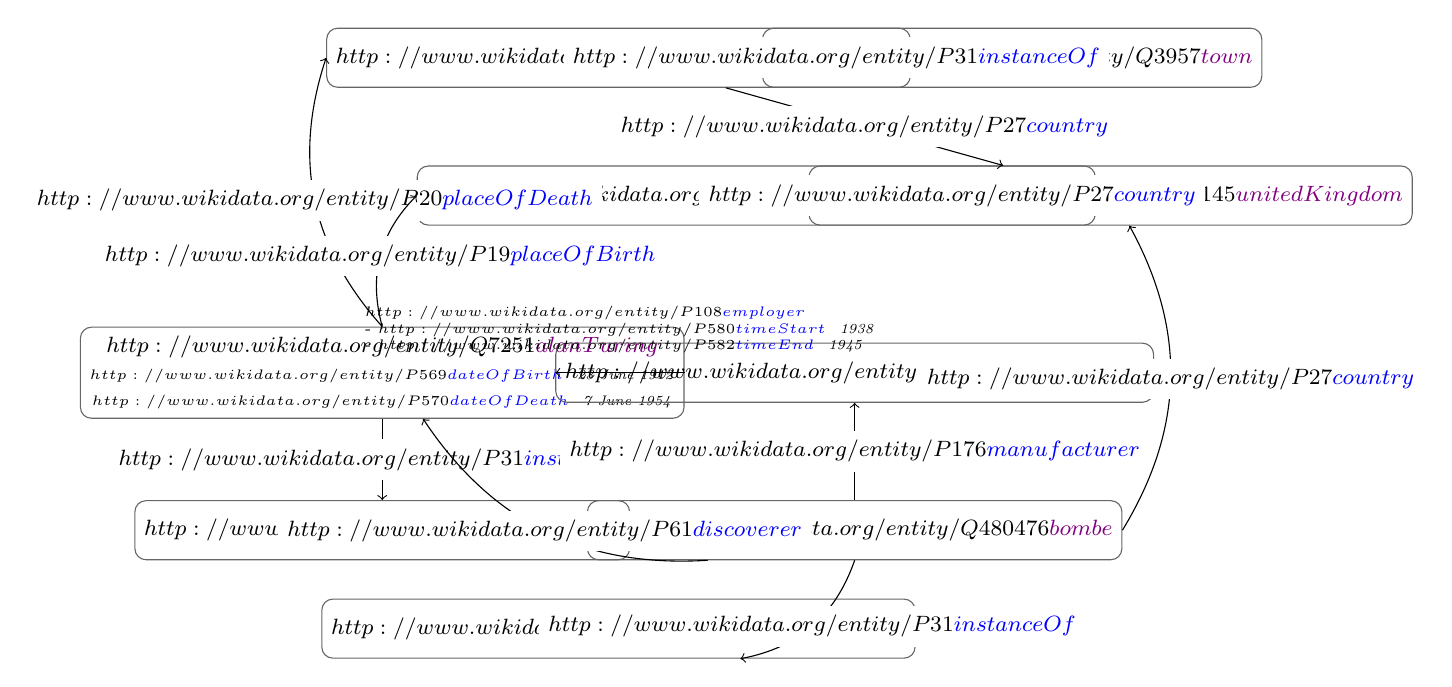
\begin{tikzpicture}[
        vertex/.style={rectangle, rounded corners, draw=black!60, minimum width=15mm, minimum height=7.5mm, text centered, font=\footnotesize},
        predicate/.style = {fill=white, font=\footnotesize}
    ]
    \node[vertex,align=center] (alanTuring) at (-2, 0) {\alanTuring\\{\tiny \dateOfBirth  \hspace{1mm} \textit{23 June 1912}}\\{\tiny \dateOfDeath  \hspace{1mm} \textit{7 June 1954}}};
    \node[vertex] (human) at (-2, -2) {\Human};
    \node[vertex] (birth) at (2.75, 2.25) {\warringtonLodge};
    \node[vertex] (death) at (1, 4) {\wilmslow};
    \node[vertex] (employer) at (4, 0) {\government};
    \node[vertex] (country) at (7.25, 2.25) {\unitedKingdom};
    \node[vertex] (bombe) at (4, -2) {\bombe};
    \node[vertex] (machine) at (1, -3.25) {\computer};
    \node[vertex] (town) at (6, 4) {\town};

    \path[-to] (alanTuring.north) edge[bend left] node[predicate] {\placeOfDeath} (death.west);
    \path[-to] (alanTuring.north) edge[bend left] node[predicate] {\placeOfBirth} (birth.west);
    \path[-to] (alanTuring.south) edge node[predicate] {\instanceOf} (human.north);
    \path[-to] (alanTuring.east) edge node[label={[align=left,font=\tiny]above:\employer\\- \timeStart \hspace{1mm} \textit{1938}\\- \timeEnd \hspace{1mm} \textit{1945}}] {} (employer.west);
    \path[-to] (birth.east) edge node[predicate] {\country} (country.west);
    \path[-to] (bombe.south) edge[bend left] node[predicate] {\instanceOf} (machine);
    \path[-to] (bombe.north) edge node[predicate] {\manufacturer} (employer.south);
    \path[-to] (bombe) edge[bend left] node[predicate] {\discoverer} (alanTuring);
    \path[-to] (bombe.east) edge[bend right] node[predicate] {\country} (country);
    \path[-to] (death.east) edge node[predicate] {\instanceOf} (town.west);
    \path[-to] (death) edge node[predicate] {\country} (country);
\end{tikzpicture}
\end{document}